\documentclass[a4paper,twocolumn,11pt]{quantumarticle}
\pdfoutput=1

\usepackage[utf8]{inputenc}
\usepackage[english]{babel}

\usepackage[numbers,sort&compress]{natbib}
\bibliographystyle{plainnat}

\usepackage[T1]{fontenc}
\usepackage{amsmath}
\usepackage{amsfonts}
\usepackage{hyperref}

\usepackage{tikz}
\usepackage{lipsum}
\usepackage[printonlyused,withpage]{acronym}
\usepackage{braket}
\usepackage{mathtools}
\usepackage{array, multirow, bigdelim, makecell, booktabs}
\usepackage{qcircuit}
\usepackage{blochsphere}
\usepackage{stackengine}
\usepackage{amssymb}
\usepackage{epigraph}
\usepackage{float}

\usetikzlibrary{arrows, shapes, shapes.multipart, trees, positioning,
    backgrounds, fit, matrix, external, 
    positioning, arrows, calc, math, angles, quotes, babel, arrows.meta}

\definecolor{rbeige}{HTML}{F7EFE5}
\definecolor{rblue1}{HTML}{D0BFFF}
\definecolor{rblue2}{HTML}{C3ACD0}
\definecolor{rblue3}{HTML}{7743DB}
\definecolor{rred}{HTML}{FA7070}
\definecolor{rgreen}{HTML}{A5DD9B}
\definecolor{rpink}{HTML}{FA4EAB}
\definecolor{rgray}{HTML}{DDDDDD}

\def\hyph{-\penalty0\hskip0pt\relax}

\begin{document}

\title{{An Incomplete Introduction to Quantum Error Correction}}
\author{Matthias Reumann}
\affiliation{Technische Universität München, Munich, Germany}
\email{matthias.reumann@tum.de}
\maketitle

\begin{abstract}
    Quantum Error Correction is an essential building block towards {Fault-Tolerant} Quantum Computing. This paper introduces the theoretical minimum required for the former and briefly introduces the latter. We do so in a beginner-friendly and graphically-supplemented fashion.
\end{abstract}

\section{Introduction}

Quantum computing is a hot topic. Feynman's dreams of a quantum computer in 1982~\cite{feynman1982simulating} are today's promises of companies such as IBM, Google, and Microsoft~\cite{ibm_ibm_2024,google_quantum_ai_our_2024,azure_quantum_2024}. The ultimate goal is to run algorithms on these hardware devices. Similar to World War 2, applications in cryptography demonstrate the usefulness of quantum computing technology~\cite{preskill_quantum_2023}. Namely, Shor's prime factoring algorithm and its consequences on current cryptographic systems~\cite{shor_factoring_1997}. Over time, a wide range of algorithms with speed-ups over their classical counterparts emerged. Another critical field of research lies between the advancements in quantum hardware and the invention of quantum algorithms: quantum error correction. Its task is to protect delicate qubits from the adverse effects of errors. Error sources include qubit\hyph{}environment interactions, so-called \textit{decoherence}, and faulty gates.

In this paper, we review the fundamental concepts of quantum error correction in an intuitive and easily digestible way. For the content we primarily rely on already existing, but math-heavy, introductions such as Ref.~\cite{gottesman_introduction_2009} and textbooks such as Ref.~\cite{nielsen00}. Nevertheless, we always reference source materials as well as contemporary research results for a deeper dive into the literature. A main achievement of this paper is the supplementation of existing resources with graphical intuition.
\section{Challenges}

Even though quantum error correction often borrows ideas from its classical counterpart, quantum error correction faces the following unique challenges.

\vspace{0.75em}
\noindent
\textbf{No-Cloning Theorem} The no-cloning theorem states that no unitary operation $U$ exists that copies an unknown quantum state $\ket{\psi}$. Consequently, quantum analogs of classical repetition codes, where one copies individual bits and takes a majority vote, are infeasible.
\begin{equation*}
    \Qcircuit @C=1.5em @R=1em {
        \lstick{\ket{\psi}}  & \multigate{1}{U}  & \rstick{\ket{\psi}} \qw \\ 
        \lstick{\ket0}       & \ghost{U}         & \rstick{\ket{\psi}} \qw }
\end{equation*}

\vspace{0.5em}
\noindent
\textbf{Continous Errors} A qubit can be in any superposition of the basis states $\ket{0}$ and $\ket{1}$.
\begin{equation}
    \alpha\ket{0} + \beta\ket{1}
\end{equation}
where $\alpha{}$ and $\beta{}$ are complex numbers that fulfill the constraint $|\alpha{}|^2 + |\beta{}|^2 = 1$. Thus, a quantum computer has a continuum of states. Ordinary classical computers are binary - a bit is either $0$ or $1$, even after a bit-flip error. In comparison, it seems like quantum error correction requires an infinite amount of precision to detect all possible errors.

Let's look at a concrete and practically relevant example. Imagine that a quantum computer implements the following rotation operation.
\begin{equation}
    \begin{pmatrix}
        1 & 0 \\
        0 & e^{i\theta}
    \end{pmatrix}
\end{equation}
However, due to some miscalibration, it ends up rotating not by $\theta$ but $\theta{}+\delta{}$. Figure~\ref{fig:continous-errors} depicts this scenario on the \textit{bloch sphere} for a $\frac{\pi}{2}$ rotation. Throughout the computation, we apply this faulty operation many times. How small $\delta$ may be, the accumulation of errors ultimately leads to inaccurate results. A reasonable idea therefore is to detect and correct this error. The difficulty lies in the fact that $\delta$ can be any real number, leaving us with the problem stated in the previous paragraph.

\begin{figure}[h]
    \centering
    \begin{blochsphere}[radius=2cm,opacity=0,rotation=-105]
        \coordinate (origin) at (0,0);

        \drawLongitudeCircle[]{-105};
        \drawLatitudeCircle[style={opacity=0.4, dashed, thin}]{0};
        
        \labelLatLon{ket0}{90}{0};
        \labelLatLon{ket1}{-90}{0};
        \labelLatLon{ketminus}{0}{180};
        \labelLatLon{ketplus}{0}{0};

        \labelLatLon{ketplusi}{0}{-90};
        \labelLatLon{ketminusi}{0}{-270};

        \labelLatLon{ketpluserror}{0}{-25};

        \draw[opacity=0.4, dashed, thin] (ket0) -- (ket1);
        \draw[opacity=0.4, dashed, thin] (ketplus) -- (ketminus);
        \draw[opacity=0.4, dashed, thin] (ketplusi) -- (ketminusi);

        \node[above, inner sep=.25em] at (ket0) {\footnotesize$\ket0$};
        \node[below, inner sep=.25em] at (ket1) {\footnotesize$\ket1$};
        
        { 
            \setDrawingPlane{0}{0}
            \pic["\footnotesize $\frac{\pi}{2}$", current plane, draw, fill=rblue2!50, fill opacity=.5, text opacity=1, angle radius=2.2em, angle eccentricity=1.3,-Straight Barb]{angle=ketminus--origin--ketplus};
            \pic["\footnotesize $\delta$", current plane, draw, fill=rred!50, fill opacity=.5, text opacity=1, angle radius=2.2em,angle eccentricity=1.75]{angle=ketplus--origin--ketpluserror};
            
        }
        
        \draw[color=black, -latex] (origin) -- (ketpluserror);
    \end{blochsphere}
    \caption{Over-rotation by $\delta$ for a desired $\frac{\pi}{2}$ rotation on the bloch sphere.}\label{fig:continous-errors}
\end{figure}

\vspace{0.5em}
\noindent
\textbf{Measurements destroy quantum information} Measurements in quantum mechanics destroy the superposition of a quantum state. Contrary to the classical approach, we can not recover the original superposition after observing the state.

\smallskip
\noindent
Given these three challenges, quantum error correction seems like a daunting, if not impossible, task. Fortunately, as we will illustrate in the succeeding sections, each challenge can be overcome.
\section{Physical \& Logical Qubits}

By the rules of quantum mechanics, we can't utilize redundancy in the form of repetition codes to protect qubits. However, there are also phenomenons with no classical equivalent such as entanglement. In 1995, Shor was one of the first to take advantage of this quantum effect for quantum error correction.
\begin{figure}[h]
    \centering
    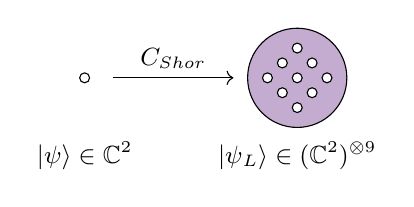
\begin{tikzpicture}[scale=.9]
    
    \filldraw [color=black, fill=white, thin] (0,0) circle (0.07);

    \draw[thin, ->] (0.4,0) -- (2.1,0) node[midway, above] {\small $C_{Shor}$};    

    \filldraw [color=black, fill=rblue2, thin] (3,0) circle (0.7);

    \filldraw [color=black, fill=white, thin] (3,0) circle (0.07);
    \filldraw [color=black, fill=white, thin] (3,0.42) circle (0.07);
    \filldraw [color=black, fill=white, thin] (3.21,0.21) circle (0.07);
    \filldraw [color=black, fill=white, thin] (3.42,0) circle (0.07);
    
    \filldraw [color=black, fill=white, thin] (2.79,0.21) circle (0.07);

    \filldraw [color=black, fill=white, thin] (2.79,-0.21) circle (0.07);
    \filldraw [color=black, fill=white, thin] (2.58, 0) circle (0.07);
    \filldraw [color=black, fill=white, thin] (3, -0.42) circle (0.07);
    \filldraw [color=black, fill=white, thin] (3.21,-0.21) circle (0.07);

    
    \node at (0,-1.1) {\small $\ket{\psi}\in\mathbb{C}^{2}$};
    \node at (3, -1.1) {\small $\ket{\psi{}_L}\in(\mathbb{C}^{2})^{\otimes{}9}$};
    
    
    
    \end{tikzpicture}
    \caption{Encoding of one physical qubit $\ket{\psi}$ into one logical qubit $\ket{\psi_L}$. The logical qubit entangles multiple physical qubits.}\label{fig:physical_to_logical_qubit}
\end{figure}

\noindent
The Shor code stores the information of a single \textit{logical} qubit in the entanglement between nine \textit{physical} ones~\cite{shor_scheme_1995}. Consequently, no specific (possibly faulty) qubit stores all the state's information. Figure~\ref{fig:physical_to_logical_qubit} depicts this procedure schematically. The underlying idea is borrowed from classical codes: Use many to protect the few. But entangle qubits instead of cloning.

Equations~\ref{eq:shor-logical-0}-\ref{eq:shor-logical-1} define the Shor code and its logical qubits mathematically. Notice that the qubit triplet in the brackets is the Greenberger-Horne-Zeilinger (GHZ) state, a maximally entangled state. 
\begin{equation}\label{eq:shor-logical-0}
    \ket{0_L} = \left(\frac{\ket{000}+\ket{111}}{\sqrt{2}}\right)^{\otimes{}3}
\end{equation}
\begin{equation}\label{eq:shor-logical-1}
    \ket{1_L} = \left(\frac{\ket{000}-\ket{111}}{\sqrt{2}}\right)^{\otimes{}3}
\end{equation}
\begin{equation}\label{eq:the-shor-code}
    \mathcal{Q}_{shor} = \{\ket{0_L}, \ket{1_L}\}
\end{equation}
It should be no surprise that the encoding circuit for the Shor code stacks three GHZ circuits. We refer the reader to Ref.~\cite{nguyen_demonstration_2021}, which implements the Shor code on a trapped-ion device, to validate this fact.
\section{Pauli matrices \& the Pauli group}\label{sec:errors}

Equations~\ref{eq:pauli-matrix-I}-\ref{eq:pauli-matrix-Z} define the famous \textit{Pauli matrices}. In the quantum circuit model, the Pauli matrices are referred to as \textit{Pauli gates}.
\begin{equation}\label{eq:pauli-matrix-I}
    \begin{aligned}
        I = \begin{pmatrix}
            1 & 0 \\
            0 & 1 \\
        \end{pmatrix} & & \text{``identity''}
    \end{aligned}
\end{equation}
\begin{equation}\label{eq:pauli-matrix-X}
    \begin{aligned}
        X = \begin{pmatrix}
            0 & 1 \\
            1 & 0 \\
        \end{pmatrix} & & \text{``bit flip''}
    \end{aligned}
\end{equation}
\begin{equation}\label{eq:pauli-matrix-Y}
    \begin{aligned}
        Y = iXZ = \begin{pmatrix}
            0 & -i \\
            i & 0 \\
        \end{pmatrix} & & \text{``bit \& phase flip''}
    \end{aligned}
\end{equation}
\begin{equation}\label{eq:pauli-matrix-Z}
    \begin{aligned}
        Z = \begin{pmatrix}
            1 & 0 \\
            0 & -1 \\
        \end{pmatrix} & & \text{``phase flip''}
    \end{aligned}
\end{equation}
A useful fact that will be of significance later is that $X$, $Y$, and $Z$ anti-commute. That is, ${XZ = -ZX}$, written as $\{X, Z\} = 0$, and similarly for any other pair.

The Pauli matrices generate the \textit{Pauli group} $\mathcal{P}_{n}$. Mathematically, it is the $n$-fold tensor product of the four Pauli matrices with factors $\pm{}1$, and $\pm{}i$. The factors are necessary to build a valid group. Any two elements of the Pauli group either commute or anti-commute, where one defines commutation as $AB = BA$ and denotes it as ${[A, B] = 0}$. 

These matrices are important because they span the space of all $2 \times 2$ matrices. Likewise, the Pauli group spans the space of $2^{n}\times 2^{n}$ matrices. Thus, any error $E$ can be expanded as a linear combination of these matrices.
\begin{equation}
    E = aI + bX + cY + dZ
\end{equation}
Now, assume a single-qubit error occurs on the first qubit of many. The resulting state $E_{1}\ket{\psi}$ is also a linear combination of the terms $I_{1}\ket{\psi}$, $X_{1}\ket{\psi}$, $Y_{1}\ket{\psi}$, and $Z_{1}\ket{\psi}$. Then, after a measurement, the state would collapse to one of these terms. If we knew with which term we ended up, we could correct the error by applying the respective Pauli gate. In the next section, we introduce a formalism that underlies most of today's quantum codes and enables such a detection mechanism.
\section{The Stabilizer Formalism}\label{sec:stabilizers}

The stabilizer formalism is an important tool for building modern quantum codes. Its fundamental idea resembles parity check matrices from classical coding theory. This section explores this resemblance and introduces stabilizer codes formally. Stabilizers have been pioneered by Daniel Gottesman in his Ph.D. thesis~\cite{gottesman1997stabilizer}.

\subsection{Hamming Codes}\label{subsec:hamming}

Hamming codes use parity-check matrices to calculate \textit{syndrome vectors}. 
\begin{equation}
    s = Hx\pmod{2}
\end{equation}
If a syndrome vector $s$ equals zero, no error occurred. Otherwise, $s$ indicates which bit has been flipped. Equation~\ref{eq:hamming-parity-matrix} shows the parity-check matrix $H$ for the $[7,4,3]$ code.
\begin{equation}
    H = 
    \begin{pmatrix}
        r_1 \\
        r_2 \\
        r_3 \\
    \end{pmatrix}
    =
    \begin{pmatrix}
        1 & 0 & 1 & 0 & 1 & 0 & 1 \\ 
        0 & 1 & 1 & 0 & 0 & 1 & 1 \\ 
        0 & 0 & 0 & 1 & 1 & 1 & 1 \\ 
    \end{pmatrix}
    \label{eq:hamming-parity-matrix}
\end{equation}
Figure~\ref{fig:hamming-rows} illustrates the {dot-product} between each row of $H$ and $x = 0111010$. Note that each dot-product $r_{i\in\{1,2,3\}}x\pmod{2}$ yields one bit of the syndrome vector and splits the codeword into a violet ($\textcolor{rblue3}\bullet{}$) and white ($\circ{}$) group. The resulting syndrome vector is $s=(1\text{ }1\text{ }0)$, or intuitively $(\textcolor{rblue3}\bullet{}$\text{ }$\textcolor{rblue3}\bullet{}$\text{ }$\circ{})$. Consequently, $s$ tells us the error is in the third bit. The corrected codeword is $\hat{x} = 0101010$.
\begin{figure}[h]
    \centering
    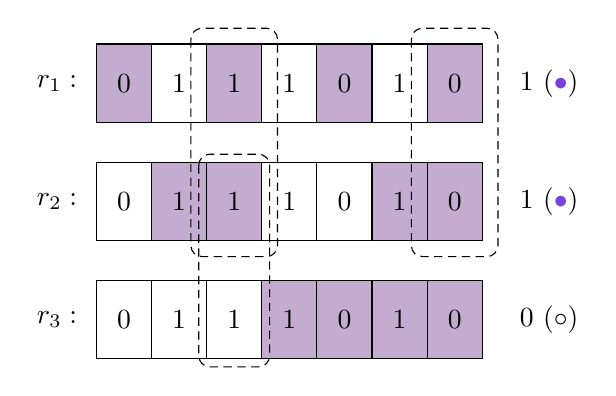
\begin{tikzpicture}[scale=1]
        
        \draw[color=black, fill=rblue2, thin] (0,0) rectangle (0.7,1) node[midway] {0};
        \draw[color=black, thin] (0.7,0) rectangle (1.4,1) node[midway] {1};
        \draw[color=black, fill=rblue2, thin] (1.4,0) rectangle (2.1,1) node[midway] {1};
        \draw[color=black, thin] (2.1,0) rectangle (2.8,1) node[midway] {1};
        \draw[color=black, fill=rblue2, thin] (2.8,0) rectangle (3.5,1) node[midway] {0};
        \draw[color=black, thin] (3.5,0) rectangle (4.2,1) node[midway] {1};
        \draw[color=black, fill=rblue2, thin] (4.2,0) rectangle (4.9,1) node[midway] {0};

        \node at (-0.5, 0.5) {$r_1:$};
        \node at (5.75, 0.5) {$1$ (\textcolor{rblue3}{$\bullet$})};

        \draw[color=black, thin] (0,-1.5) rectangle (0.7,-0.5) node[midway] {0};
        \draw[color=black, fill=rblue2, thin] (0.7,-1.5) rectangle (1.4,-0.5) node[midway] {1};
        \draw[color=black, fill=rblue2, thin] (1.4,-1.5) rectangle (2.1,-0.5) node[midway] {1};
        \draw[color=black, thin] (2.1,-1.5) rectangle (2.8,-0.5) node[midway] {1};
        \draw[color=black, thin] (2.8,-1.5) rectangle (3.5,-0.5) node[midway] {0};
        \draw[color=black, fill=rblue2, thin] (3.5,-1.5) rectangle (4.2,-0.5) node[midway] {1};
        \draw[color=black, fill=rblue2, thin] (4.2,-1.5) rectangle (4.9,-0.5) node[midway] {0};

        \node at (-0.5, -1) {$r_2:$};
        \node at (5.75, -1) {$1$ (\textcolor{rblue3}{$\bullet$})};

        
        \draw[color=black, thin]                (0,-3) rectangle (0.7,-2) node[midway] {0};
        \draw[color=black, thin]                (0.7,-3) rectangle (1.4,-2) node[midway] {1};
        \draw[color=black, thin]                (1.4,-3) rectangle (2.1,-2) node[midway] {1};
        \draw[color=black, fill=rblue2, thin]   (2.1,-3) rectangle (2.8,-2) node[midway] {1};
        \draw[color=black, fill=rblue2, thin]   (2.8,-3) rectangle (3.5,-2) node[midway] {0};
        \draw[color=black, fill=rblue2, thin]   (3.5,-3) rectangle (4.2,-2) node[midway] {1};
        \draw[color=black, fill=rblue2, thin]   (4.2,-3) rectangle (4.9,-2) node[midway] {0};

        \node at (-0.5, -2.5) {$r_3:$};
        \node at (5.75, -2.5) {$0$ ($\circ$)};

        
        \draw[color=black, densely dashed, thin, rounded corners=4pt] (1.2,1.2) rectangle (2.3,-1.7);
        \draw[color=black, densely dashed, thin, rounded corners=4pt] (4, 1.2) rectangle (5.1,-1.7);
        \draw[color=black, densely dashed, thin, rounded corners=4pt] (1.3,-0.4) rectangle (2.2,-3.1);

        
        
        

        
        

        
        
        
        

        
        

        
        

        
    \end{tikzpicture}

    \caption{Application of the parity check matrix $H_{[7,4,3]}$ on $0111010$ and the resulting syndrome vector $(1\text{ }1\text{ }0)$. The overlap of the dashed rectangles illustrates the error detection procedure.}\label{fig:hamming-rows}
\end{figure}

\subsection{Stabilizer Codes}

A matrix $M\in\mathcal{P}_n$ stabilizes the state $\ket{\psi}$ if $M\ket{\psi} = +1\ket{\psi}$. In other words, $\ket{\psi}$ is an eigenvector of $M$ with eigenvalue $+1$. The states stabilized by a set $S$ of commuting matrices $M_{i}$ define the codewords of a quantum code $\mathcal{Q}$, where $-I \notin S$.
\begin{equation}\label{eq:stabilizer}
    \mathcal{Q} = \{\ket{\psi} : M_{i}\ket{\psi} = \ket{\psi}, \forall{}M_{i} \in S\}
\end{equation}
Remember that in Section~\ref{sec:errors} we learned that any two elements of the Pauli group either commute or anti-commute. Furthermore, we can assume that $E\in\mathcal{P}_{n}$. Hence, either Equation~\ref{eq:stabilizers-error-commute} or Equation~\ref{eq:stabilizers-error-anticommute} holds.
\begin{equation}\label{eq:stabilizers-error-commute}
    M_{i}(E\ket{\psi}) = EM_{i}\ket{\psi} = +1(E\ket{\psi})
\end{equation}
\begin{equation}\label{eq:stabilizers-error-anticommute}
    M_{i}(E\ket{\psi}) = -EM_{i}\ket{\psi} = -1(E\ket{\psi})
\end{equation}
Using this fact, we define the syndrome $s = (s_{1},s_{2},\ldots, s_{|S|})$ associated with an error $E$ is as follows.
\begin{equation}
    s_{i} = \begin{cases}
            0 & \text{ if }[E, M_{i}] = 0\\ 
            1 & \text{ if }\{E, M_{i}\} = 0\end{cases}
\end{equation}
This tells us that we can detect any error $E$ if we measure a set of carefully chosen stabilizers $M_{i}$.

\smallskip 

\noindent
Let's return to the Shor code. Namely, its stabilizers as defined in Table~\ref{table:shor-stabilizers}. For brevity, we have omitted the Kronecker product between the Pauli matrices. The \textit{weight} of a stabilizer is the amount of non-trivially acting Pauli matrices, e.g. $wt(M_7) = 6$. Furthermore, using Equation~\ref{eq:stabilizer} we can alternatively define the logical states of the Shor code in terms of these stabilizers. That is, $\{\ket{\psi} : M_{i}\ket{\psi} = \ket{\psi}\} = \mathcal{Q}_{shor}$.

\begin{table}[h]
    \centering
    \resizebox{\columnwidth}{!}{%
    \begin{tabular}{cccccccccc}
        & {\scriptsize $1$} & {\scriptsize $2$} & {\scriptsize $3$} & {\scriptsize $4$} & {\scriptsize $5$} & {\scriptsize $6$}& {\scriptsize $7$} & {\scriptsize $8$}& {\scriptsize $9$}\\
        $M_1 = $ & $Z$ & $Z$ & $I$ & $I$ & $I$ & $I$ & $I$ & $I$ & $I$ \\
        $M_2 = $ & $I$ & $Z$ & $Z$ & $I$ & $I$ & $I$ & $I$ & $I$ & $I$ \\
        $M_3 = $ & $I$ & $I$ & $I$ & $Z$ & $Z$ & $I$ & $I$ & $I$ & $I$ \\
        $M_4 = $ & $I$ & $I$ & $I$ & $I$ & $Z$ & $Z$ & $I$ & $I$ & $I$ \\
        $M_5 = $ & $I$ & $I$ & $I$ & $I$ & $I$ & $I$ & $Z$ & $Z$ & $I$ \\
        $M_6 = $ & $I$ & $I$ & $I$ & $I$ & $I$ & $I$ & $I$ & $Z$ & $Z$ \\
        $M_7 = $ & $X$ & $X$ & $X$ & $X$ & $X$ & $X$ & $I$ & $I$ & $I$ \\
        $M_8 = $ & $I$ & $I$ & $I$ & $X$ & $X$ & $X$ & $X$ & $X$ & $X$ \\
    \end{tabular}
    }
    \caption{The eight stabilizers for the Shor code. Kronecker products between Pauli matrices omitted for brevity.}\label{table:shor-stabilizers}
\end{table}

\noindent
Each measurement of a stabilizer yields one syndrome bit. Combining the information of all measurements tells us not only if an error happened but also which one and where. Let us walk through a simple example to see this procedure in action. Let $\ket{x}$ be the $\ket{0_L}$ codeword, where we bit-flip the third qubit:
\begin{equation}
    \left(\frac{\ket{00\textcolor{purple}{1}}+\ket{11\textcolor{purple}{0}}}{\sqrt{2}}\right)\otimes\left(\frac{\ket{000}+\ket{111}}{\sqrt{2}}\right)^{\otimes{}2}
\end{equation}
The measurement of all stabilizers $M_1$ to $M_8$ yields syndrome vector
\begin{equation}
    s=(0\text{ }1\text{ }0\text{ }0\text{ }0\text{ }0\text{ }0\text{ }0)
\end{equation}
or alternatively {color-coded} $(\circ{}\text{ }\textcolor{rblue3}\bullet{}\text{ }\circ{}\text{ }\circ{}\text{ }\circ{}\text{ }\circ{}\text{ }\circ{}\text{ }\circ{})$. A few observations follow. First of all, because it is not the zero vector some error occurred. Secondly, $M_2$ is the only stabilizer acting non-trivially on $\ket{x}$ which results in a syndrome bit of $1$. Lastly, as with classical parity checks combining the information of all syndrome bits tells us that an $X$ error occurred on the third qubit. Thus, applying a $X$ gate on the third qubit corrects the error. Figure~\ref{fig:synd-msmt} depicts this procedure graphically. A comparison to Figure~\ref{fig:hamming-rows} might be illuminating. We leave it up to the reader to validate this procedure for $Y$ and $Z$ errors.

\begin{figure*}
    \centering
    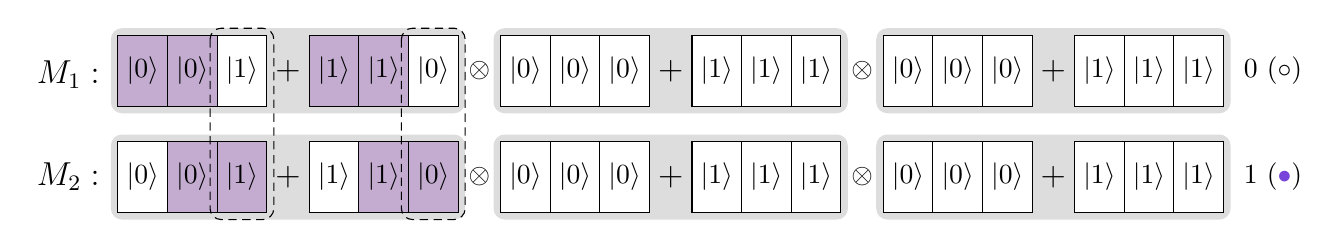
\begin{tikzpicture}[scale=0.9]
        \node at (-0.7, 0.45) {\large$M_{1}:$};
        
        
        \fill[color=rgray, rounded corners=4pt] (-0.1, -0.1) rectangle (4.9, 1.1);
        \draw[color=black, fill=rblue2, thin] (0.0,0) rectangle (0.7,1) node[midway] {\textcolor{black}{$\ket{0}$}};
        \draw[color=black, fill=rblue2, thin] (0.7,0) rectangle (1.4,1) node[midway] {\textcolor{black}{$\ket{0}$}};
        \draw[color=black, fill=white, thin] (1.4,0) rectangle (2.1,1) node[midway] {\textcolor{black}{$\ket{1}$}};

        \node at (2.4, 0.5) {\large$+$};

        \draw[color=black, fill=rblue2, thin] (2.7,0) rectangle (3.4,1) node[midway] {\textcolor{black}{$\ket{1}$}};
        \draw[color=black, fill=rblue2, thin] (3.4,0) rectangle (4.1,1) node[midway] {\textcolor{black}{$\ket{1}$}};
        \draw[color=black, fill=white, thin] (4.1,0) rectangle (4.8,1) node[midway] {\textcolor{black}{$\ket{0}$}};

        \node at (5.1, 0.5) {$\otimes$};

        \fill[color=rgray, rounded corners=4pt] (5.3, -0.1) rectangle (10.3, 1.1);
        \draw[color=black, fill=white, thin] (5.4,0) rectangle (6.1,1) node[midway] {$\ket{0}$};
        \draw[color=black, fill=white,thin] (6.1,0) rectangle (6.8,1) node[midway] {$\ket{0}$};
        \draw[color=black, fill=white,thin] (6.8,0) rectangle (7.5,1) node[midway] {$\ket{0}$};

        \node at (7.8, 0.5) {\large$+$};

        \draw[color=black, fill=white,thin] (8.1, 0) rectangle (8.8,1) node[midway] {$\ket{1}$};
        \draw[color=black, fill=white,thin] (8.8,0) rectangle (9.5,1) node[midway] {$\ket{1}$};
        \draw[color=black, fill=white,thin] (9.5,0) rectangle (10.2,1) node[midway] {$\ket{1}$};

        \node at (10.5, 0.5) {$\otimes$};

         
        \fill[color=rgray, rounded corners=4pt] (10.7, -0.1) rectangle (15.7, 1.1);
        \draw[color=black, fill=white,thin] (10.8,0) rectangle (11.5,1) node[midway] {$\ket{0}$};
        \draw[color=black, fill=white,thin] (11.5,0) rectangle (12.2,1) node[midway] {$\ket{0}$};
        \draw[color=black, fill=white,thin] (12.2,0) rectangle (12.9,1) node[midway] {$\ket{0}$};

        \node at (13.2, 0.5) {\large$+$};

        \draw[color=black, fill=white,thin] (13.5,0) rectangle (14.2,1) node[midway] {$\ket{1}$};
        \draw[color=black, fill=white,thin] (14.2,0) rectangle (14.9,1) node[midway] {$\ket{1}$};
        \draw[color=black, fill=white,thin] (14.9,0) rectangle (15.6,1) node[midway] {$\ket{1}$};

        \node at (16.3, 0.5) {$0$ ($\circ$)};
        
        
        
        \node at (-0.7, -1) {\large$M_{2}:$};

        
        \fill[color=rgray, rounded corners=4pt] (-0.1, -1.6) rectangle (4.9, -0.4);
        \draw[color=black, fill=white,thin] (0.0,-1.5) rectangle (0.7,-0.5) node[midway] {\textcolor{black}{$\ket{0}$}};
        \draw[color=black, fill=rblue2, thin] (0.7,-1.5) rectangle (1.4,-0.5) node[midway] {\textcolor{black}{$\ket{0}$}};
        \draw[color=black, fill=rblue2, thin] (1.4,-1.5) rectangle (2.1,-0.5) node[midway] {\textcolor{black}{$\ket{1}$}};

        \node at (2.4, -1) {\large$+$};

        \draw[color=black, fill=white,thin] (2.7,-1.5) rectangle (3.4,-0.5) node[midway] {\textcolor{black}{$\ket{1}$}};
        \draw[color=black, fill=rblue2, thin] (3.4,-1.5) rectangle (4.1,-0.5) node[midway] {\textcolor{black}{$\ket{1}$}};
        \draw[color=black, fill=rblue2, thin] (4.1,-1.5) rectangle (4.8,-0.5) node[midway] {\textcolor{black}{$\ket{0}$}};

        \node at (5.1, -1) {$\otimes$};

        
        \fill[color=rgray, rounded corners=4pt] (5.3, -1.6) rectangle (10.3, -0.4);
        \draw[color=black, fill=white,thin] (5.4,-1.5) rectangle (6.1,-0.5) node[midway] {$\ket{0}$};
        \draw[color=black, fill=white,thin] (6.1,-1.5) rectangle (6.8,-0.5) node[midway] {$\ket{0}$};
        \draw[color=black, fill=white,thin] (6.8,-1.5) rectangle (7.5,-0.5) node[midway] {$\ket{0}$};

        \node at (7.8, -1) {\large$+$};

        \draw[color=black, fill=white,thin] (8.1, -1.5) rectangle (8.8,-0.5) node[midway] {$\ket{1}$};
        \draw[color=black, fill=white,thin] (8.8,-1.5) rectangle (9.5,-0.5) node[midway] {$\ket{1}$};
        \draw[color=black, fill=white,thin] (9.5,-1.5) rectangle (10.2,-0.5) node[midway] {$\ket{1}$};

        \node at (10.5, -1) {$\otimes$};

        
        \fill[color=rgray, rounded corners=4pt] (10.7, -1.6) rectangle (15.7, -0.4);
        \draw[color=black, fill=white,thin] (10.8,-1.5) rectangle (11.5,-0.5) node[midway] {$\ket{0}$};
        \draw[color=black, fill=white,thin] (11.5,-1.5) rectangle (12.2,-0.5) node[midway] {$\ket{0}$};
        \draw[color=black, fill=white,thin] (12.2,-1.5) rectangle (12.9,-0.5) node[midway] {$\ket{0}$};

        \node at (13.2, -1) {\large$+$};

        \draw[color=black, fill=white,thin] (13.5,-1.5) rectangle (14.2,-0.5) node[midway] {$\ket{1}$};
        \draw[color=black, fill=white,thin] (14.2,-1.5) rectangle (14.9,-0.5) node[midway] {$\ket{1}$};
        \draw[color=black, fill=white,thin] (14.9,-1.5) rectangle (15.6,-0.5) node[midway] {$\ket{1}$};

        \node at (16.3, -1) {$1$ (\textcolor{rblue3}{$\bullet$})};

        
        \draw[color=black, densely dashed, thin, rounded corners=4pt] (1.3,1.1) rectangle (2.2,-1.6);
        \draw[color=black, densely dashed, thin, rounded corners=4pt] (4,1.1) rectangle (4.9,-1.6);
    \end{tikzpicture}
    \caption{Syndrome measurement of the stabilizers $M_{1}$ and $M_{2}$ on the $\ket{0_L}$ state for the Shor code where the third qubit has been bit-flipped.}\label{fig:synd-msmt}
\end{figure*}

\subsection{Degenerate Codes}

A quantum code is \textit{degenerate} if two distinct errors $E$ and $F$ have the same syndrome vector. Otherwise, we call it \textit{non-degenerate}. 

\smallskip

\noindent
A stabilizer code is degenerate if $E^{\dagger}F \in S$. Intuitively, this means that $E$ and $F$ produce the same error on the same codeword.
\begin{equation}
    \begin{aligned}
        \ket{err} &= F\ket{\psi_{L}} = E\ket{\psi_{L}}\\
        &= E^{\dagger}F\ket{\psi_{L}} = E^{\dagger}E\ket{\psi_{L}} \\
        &= (E^{\dagger}F)\ket{\psi_{L}} = \ket{\psi_{L}}
    \end{aligned}
\end{equation}
For example, it is easy to see that a $Z_{1}$, $Z_{2}$, and $Z_{3}$ error leads to the same erroneous state for the Shor code. Moreover, $Z_{1}Z_{2}$, $Z_{2}Z_{3}$, and $Z_{1}Z_{3}$ are indeed stabilizers. Hence, the Shor code is degenerate. Interestingly, applying $Z_1$ (or $Z_2$ or $Z_3$) corrects each of these errors. This leads to the conclusion that degenerate codes can correct more errors than they can uniquely identify. Remarkably, this property is unknown to classical codes.

\subsection{Syndrome Measurements}

Each measurement of a stabilizer $M_{i}$ tells us one bit of the error syndrome. But how exactly can we measure stabilizers non-destructively?

\smallskip
\noindent
The idea is the following. First, encode the error syndrome on additional qubits, called \textit{ancilla qubits} without disturbing the actual \textit{data qubits}. Then, measure the ancilla qubits and evaluate the error syndrome.
\begin{figure}[H]
    \[
        \Qcircuit @C=1.5em @R=0.7em {
            \lstick{\ket0}      & \gate{H}  & \ctrl{1}         & \gate{H}   & \meter   & \rstick{s_i}\cw \\ 
            \lstick{}           &  \qw      & \multigate{2}{M_{i}}              & \qw        & \qw & \qw\inputgroupv{2}{4}{1em}{1.75em}{\ket{\psi}} \\
                                &  \qw      & \ghost{P}                     & \qw        & \qw & \qw \\ 
                                &  \qw      & \ghost{P}                     & \qw        & \qw & \qw \\
        }
    \]
    \caption{The phase-kickback circuit.}\label{fig:phase-kickback}
\end{figure}
\noindent
The most straightforward way of achieving this is using a \textit{phase kickback} construction. We depict its circuit in Figure~\ref{fig:phase-kickback}. The {controlled-$M_i$} gate can be constructed from multiple {controlled-$P_{i}$} gates, where $P_{i}$ is a Pauli gate acting on the $i$th qubit. Notice that the state after the controlled operation is
\begin{equation}
    \frac{\ket{0}\ket{\psi} + \ket{1}M_{i}\ket{\psi}}{\sqrt{2}}.
\end{equation}
Without an error, we can rewrite this state by using the fact that $M$ stabilizes $\ket{\psi}$.
\begin{equation}
    \frac{\ket{0}\ket{\psi} + \ket{1}\ket{\psi}}{\sqrt{2}} = \ket{+}\ket{\psi}
\end{equation}
A measurement of the ancilla qubit in the Hadamard basis reveals that the error syndrome bit for this stabilizer is $0$. Similarly, for an erroneous state and an appropriate stabilizer, the same measurement gives us a syndrome bit of $1$.
\begin{equation}
    \frac{\ket{0}(E\ket{\psi}) - \ket{1}(E\ket{\psi})}{\sqrt{2}} = \ket{-}(E\ket{\psi})
\end{equation}
Unfortunately, this procedure isn't fault-tolerant. Any single-qubit error in the controlled-$M_i$ gate can propagate to the ancilla qubit or worse an error on the ancilla results in multiple errors on the data qubits. Needless to say but of course an error on the ancilla might also lead to an incorrect syndrome bit. 

\smallskip 

\noindent
It's an open research problem to find a ``good'' solution for syndrome measurements of stabilizer codes. Error correction schemes proposed by Shor, Steane, and Knill increase the total amount of qubits by the maximum weight of a code's stabilizers. Alternatively, \textit{flag error correction} requires only $d+1$ ancilla qubits, where $d$ is the distance of a given code~\cite{Chao_2020}.

\subsection{Logical Gates}

At the end of the day, we want to run circuits to perform some kind of computation. However, so far we have only talked about the encoding of logical qubits and how to detect errors on the underlying physical qubits. For computation on logical qubits, we require \textit{logical gates}. A logical gate acts on a logical qubit and takes a valid codeword to another valid codeword. For example, a $X_{L}$ gate takes the $\ket{0_L}$ state to $\ket{1_L}$ exactly the same way as a $X$ gate takes $\ket{0}$ to $\ket{1}$.

In the stabilizer formalism, a logical gate is a matrix $U$ that commutes with all stabilizers $M_i$. Define the set of all such $U$'s as $N(S)$ and call it the \textit{normalizer} of $S$.
\begin{equation}
    M_{i}(U\ket{\psi}) = UM_{i}\ket{\psi} = U\ket{\psi}\label{eq:stabilizers-logical-operators}
\end{equation}
Thus, $U$ takes a codeword $\ket{\psi} \in \mathcal{Q}$ to another valid codeword $U\ket{\psi} \in \mathcal{Q}$. Since $U \in S$ takes any codeword to itself, we define the set of logical gates as $N(S) \backslash S$.

Going back to the Shor code, it is easily verifiable that the logical gates in Equations~\ref{eq:shor-logical-x}-\ref{eq:shor-logical-z} act like their physical counterparts.
\begin{equation}\label{eq:shor-logical-x}
    X_L = \bigotimes_{i=1}^{9}Z_{i}
\end{equation}
\begin{equation}\label{eq:shor-logical-z}
    Z_L = \bigotimes_{i=1}^{9}X_{i}
\end{equation}
Moreover, Equation~\ref{eq:stabilizers-logical-operators} also tells us that these logical gates are not unique since we can always apply stabilizers $M_i$ to $X_L$ or $Z_L$.
\begin{equation}
    \begin{aligned}
        (Z_{1}Z_{4}Z_{7})\ket{\psi} &= (M_{2}M_{4}M_{6}X_{L})\ket{\psi} \\
        &= X_{L}M_{2}M_{4}M_{6}\ket{\psi} \\
        &= X_{L}\ket{\psi}
    \end{aligned}
\end{equation}
Consequently, $Z_{1}Z_{4}Z_{7}$ is an alternative representation of the $X_L$ gate defined in Equation~\ref{eq:shor-logical-x} that uses three instead of nine physical $Z$ gates. This begs the question if there is an ``implementation'' with less than three physical gates. As it turns out, this isn't possible. For Shor's code, three is the smallest number of physical gates required to take one codeword to another. We call this smallest number the \textit{distance} of a code. This brings us finally to the classification of Shor's code. Namely, it is a $[[9,1,3]]$ quantum code, encoding $9$ physical qubits into $1$ logical qubit with a distance of $3$.
\section{Universal Quantum Computing}\label{sec:uqc}

Similarly to classical computers, where any gate can be constructed by the universal logic gates $NAND$ and $NOR$, we require a \textit{universal gate set} for quantum computers. Any unitary can be approximated in arbitrary precision by circuits constructed from this gate set~\cite{nielsen00}.

\subsection{Clifford Gates}

The Clifford gates are the unitary matrices $H$, $S$, and $CNOT$.
\begin{equation}
    H = \frac{1}{\sqrt{2}}\begin{pmatrix}
        1 & 1 \\
        1 & -1 \\
    \end{pmatrix}
\end{equation}
\begin{equation}
    S = \begin{pmatrix}
        1 & 0 \\
        0 & i \\
    \end{pmatrix}
\end{equation}
\begin{equation}
    CNOT = \begin{pmatrix}
        1 & 0 & 0 & 0 \\
        0 & 1 & 0 & 0 \\
        0 & 0 & 0 & 1 \\
        0 & 0 & 1 & 0 \\
    \end{pmatrix}
\end{equation}
These unitaries generate the Clifford group. A group of unitary matrices that map the group of Pauli matrices to itself under conjugation.
\begin{equation}
    \mathcal{C}_n = \{U : U\mathcal{P}_nU^{\dagger} = \mathcal{P}_n\}
\end{equation}
This is a special group in many ways. Firstly, the unitaries that generate it, are fundamental building blocks for many quantum algorithms, including the entanglement of two qubits. Moreover, by the definition of stabilizers as elements of the Pauli group, the Clifford group maps stabilizers to other valid stabilizers with potentially different codewords. This fact paves the way to a theorem which we briefly cover in the next section. 

\subsection{Gottesman-Knill-Theorem}

According to the Gottesman\hyph{}Knill\hyph{}Theorem, a probabilistic classical computer can efficiently simulate any circuit of Clifford gates initialized with a stabilizer state and measured in the Pauli basis~\cite{gottesman_heisenberg_1998}. Bravyi and Kitaev provide a visual addition to the theorem in~\cite{bravyi_universal_2005}. They speculate that the transition from classical computing to quantum computing occurs on the boundary of the octahedron in Figure~\ref{fig:octahedron}. As briefly mentioned before, many circuits can be constructed by the Clifford gates alone. For example, this includes the circuit for the teleportation algorithm. A full discussion of the theorem's implications does not fit here, hence, we refer the interested reader to Ref.~\cite{cuffaro_significance_2017}. Nevertheless, this beautifully shows that ``quantum supremacy'' is nuanced.
\begin{figure}[h]
    \centering
    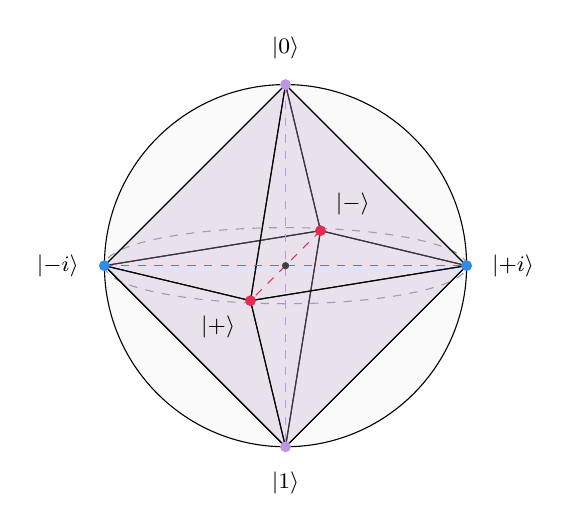
\begin{tikzpicture}[line join=bevel,z=-5.5,scale=2.3]
        \definecolor{amaranth}{rgb}{0.9, 0.17, 0.31}
        \definecolor{bleudefrance}{rgb}{0.19, 0.55, 0.91}
        \definecolor{brightlavender}{rgb}{0.75, 0.58, 0.89}

        \coordinate (B1) at (0,1,0);
        \coordinate (C1) at (0,-1,0);

        \coordinate (A1) at (0,0,-1);
        \coordinate (A3) at (0,0,1);

        \coordinate (A2) at (-1,0,0);
        \coordinate (A4) at (1,0,0);

        \filldraw[color=black, fill=gray!4](0,0) circle (1);

        
        \draw[opacity=0.4, dashed, thin] (0,0) ellipse (1 and 0.21);
        
        \draw (A1) -- (A2) -- (B1) -- cycle;
        \draw (A4) -- (A1) -- (B1) -- cycle;
        \draw (A1) -- (A2) -- (C1) -- cycle;
        \draw (A4) -- (A1) -- (C1) -- cycle;
        \draw [fill opacity=0.3,fill=rblue2] (A2) -- (A3) -- (B1) -- cycle;
        \draw [fill opacity=0.3,fill=rblue2] (A3) -- (A4) -- (B1) -- cycle;
        \draw [fill opacity=0.3,fill=rblue2] (A2) -- (A3) -- (C1) -- cycle;
        \draw [fill opacity=0.3,fill=rblue2] (A3) -- (A4) -- (C1) -- cycle;

        
        \node at (B1) [above=2mm] {\footnotesize $\ket{0}$};
        \fill [fill=brightlavender] (B1) circle (0.03);
        \draw [dashed,color=brightlavender] (B1) -- (C1);
        \node at (C1) [below=2mm] {\footnotesize $\ket{1}$};
        \fill [fill=brightlavender] (C1) circle (0.03);
        
        
        \node at (A1) [above right=1mm] {\footnotesize $\ket-$};
        \fill [fill=amaranth] (A1) circle (0.03);
        \draw [dashed,color=amaranth] (A1) -- (A3);
        \node at (A3) [below left=1mm] {\footnotesize $\ket+$};
        \fill [fill=amaranth] (A3) circle (0.03);
        
        
        \node at (A2) [left=2mm] {\footnotesize $\ket{-i}$};
        \fill [fill=bleudefrance] (A2) circle (0.03);
        \draw [dashed,color=bleudefrance] (A2) -- (A4);
        \node at (A4) [right=2mm] {\footnotesize $\ket{+i}$};
        \fill [fill=bleudefrance] (A4) circle (0.03);
    
        
        \fill [fill=darkgray] (0,0,0) circle (0.02);

        \end{tikzpicture}
    \caption{The octahedron spanned by $\ket0$ state initialization and application of the Clifford gates. Figure inspired by~\cite{azad_efficient_2024}.}\label{fig:octahedron}
\end{figure}

\subsection{The T Gate}

The Clifford gates alone do not form a universal gate set. Therefore, we need an additional non-Clifford gate to achieve this. A common choice for this non-Clifford gate is the $T$ gate. Intuitively, the $T$ gate (or any other non-Clifford) unlocks the rest of the Bloch sphere in Figure~\ref{fig:octahedron}. 
\begin{equation}
    T = \begin{pmatrix}
        1 & 0 \\
        0 & e^{i\pi{}/4} \\
    \end{pmatrix}
\end{equation}
The $T$ gate is particularly interesting because we can construct Toffoli (CCNOT) gates with it. Its textbook implementation requires seven $T$ gates~\cite{nielsen00}. However, recent work reduced that number to four~\cite{jones_novel_2013}. In turn, the importance of the Toffoli gate stems from its usage in quantum algorithms such as Shor's factoring algorithm.
\tikzset{
            logicalcnot/.pic = {
                \node at (-1, -4.75) {$CNOT_L$};
                
                {
                    
                    \draw[color=black, thin] (-2, -2.75) -- (0, -2.75);
                    \draw[color=black, fill=black, thick] (-1, -2.75) circle (0.1);
                    
                    
                    \draw[color=black, thin] (-1, -3.75) -- (-1, -2.75);
                    
                    
                    \draw[color=black, thin] (-2, -3.75) -- (0, -3.75);
                    \node at (-1, -3.75) {\Large $\oplus$};
                }
                
                
                \draw[color=black, thin] (2, 0.5) -- (7, 0.5);
                \draw[color=black, fill=black, thick] (2.4,0.5) circle (0.1);
                
                
                \draw[color=black, thin] (2, 0) -- (7, 0);
                \draw[color=black, fill=black, thick] (3.1, 0) circle (0.1);

                
                \draw[color=black, thin] (2, -0.5) -- (7, -0.5);
                \draw[color=black, fill=black, thick] (3.8, -0.5) circle (0.1);

                
                \draw[color=black, thin] (2, -1) -- (7, -1);
                \draw[color=black, fill=black, thick] (4.5, -1) circle (0.1);

                
                \draw[color=black, thin] (2, -1.5) -- (7, -1.5);
                \draw[color=black, fill=black, thick] (5.2, -1.5) circle (0.1);

                
                \draw[color=black, thin] (2, -2) -- (7, -2);
                \draw[color=black, fill=black, thick] (5.9, -2) circle (0.1);

            
                
                \draw[color=black, thin] (2, -2.5) -- (7, -2.5);
                \draw[color=black, fill=black, thick] (6.6, -2.5) circle (0.1);

                
                \draw[color=black, thin] (2.4, 0.5) -- (2.4, -4);
                \draw[color=black, thin] (3.1, 0) -- (3.1, -4.5);
                \draw[color=black, thin] (3.8, -0.5) -- (3.8, -5);
                \draw[color=black, thin] (4.5, -1) -- (4.5, -5.5);
                \draw[color=black, thin] (5.2, -1.5) -- (5.2, -6);
                \draw[color=black, thin] (5.9, -2) -- (5.9, -6.5);
                \draw[color=black, thin] (6.6, -2.5) -- (6.6, -7);

                
                
                \draw[color=black, thin] (2, -4) -- (7, -4);
                \node at (2.4, -4) {\Large $\oplus$};
                
                
                \draw[color=black, thin] (2, -4.5) -- (7, -4.5);
                \node at (3.1, -4.5) {\Large $\oplus$};

                
                \draw[color=black, thin] (2, -5) -- (7, -5);
                \node at (3.8, -5) {\Large $\oplus$};

                
                \draw[color=black, thin] (2, -5.5) -- (7, -5.5);
                \node at (4.5, -5.5) {\Large $\oplus$};

                
                \draw[color=black, thin] (2, -6) -- (7, -6);
                \node at (5.2, -6) {\Large $\oplus$};

                
                \draw[color=black, thin] (2, -6.5) -- (7, -6.5);
                \node at (5.9, -6.5) {\Large $\oplus$};

                
                \draw[color=black, thin] (2, -7) -- (7, -7);
                \node at (6.6, -7) {\Large $\oplus$};

                
                \draw[thick, -latex](0.5, -3.25) -- (1.5, -3.25);
            }
        }
\begin{figure*}
    \begin{minipage}[c]{0.6\textwidth}
        \centering
        \begin{tikzpicture}[scale=0.5,font={\footnotesize}]
            \node at (-2.5, 0.5) {\large \textbf{a}};

            \node at (-1, -4.5) {$G \in \{H,S\}$};
            \draw[color=black, thin] (-2, -3.25) -- (0, -3.25);
            \draw[color=black, fill=white, thin] (-1.5, -3.75) rectangle (-0.5,-2.75) node[midway] {$G_{L}$};
            
            
            \draw[color=black, thin] (2, 0.5) -- (4, 0.5);
            \draw[color=black, fill=white, thin] (2.5,0) rectangle (3.5,1) node[midway] {$G$};

            
            \draw[color=black, thin] (2, -0.75) -- (4, -0.75);
            \draw[color=black, fill=white, thin] (2.5,-1.25) rectangle (3.5,-0.25) node[midway] {$G$};
            
            
            \draw[color=black, thin] (2, -2) -- (4, -2);
            \draw[color=black, fill=white, thin] (2.5,-2.5) rectangle (3.5,-1.5) node[midway] {$G$};
            
            
            \draw[color=black, thin] (2, -3.25) -- (4, -3.25);
            \draw[color=black, fill=white, thin] (2.5,-3.75) rectangle (3.5,-2.75) node[midway] {$G$};

            
            \draw[color=black, thin] (2, -4.5) -- (4, -4.5);
            \draw[color=black, fill=white, thin] (2.5,-5) rectangle (3.5,-4) node[midway] {$G$};

            
            \draw[color=black, thin] (2, -5.75) -- (4, -5.75);
            \draw[color=black, fill=white, thin] (2.5,-6.25) rectangle (3.5,-5.25) node[midway] {$G$};

            
            \draw[color=black, thin] (2, -7) -- (4, -7);
            \draw[color=black, fill=white, thin] (2.5,-7.5) rectangle (3.5,-6.5) node[midway] {$G$};

            
            \draw[thick, -latex](0.5, -3.25) -- (1.5, -3.25);

            \pic[scale=0.5] at (8, 0) {logicalcnot};
        \end{tikzpicture}
    \end{minipage}
    \begin{minipage}{0.3\textwidth}
        \centering
        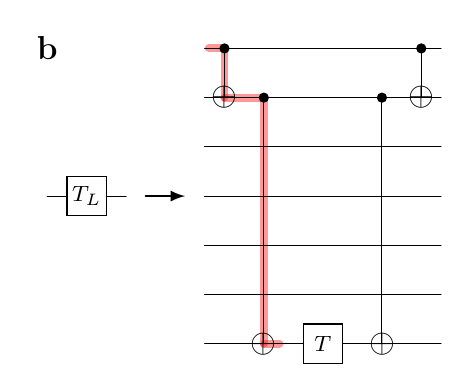
\begin{tikzpicture}[scale=0.5,font={\footnotesize},line cap=round]
            \node at (-4, 0.5) {\large \textbf{b}};

            \draw[color=black, thin] (-4, -3.25) -- (-2, -3.25);
            \draw[color=black, fill=white, thin] (-3.5, -3.75) rectangle (-2.5,-2.75) node[midway] {$T_{L}$};
            
            
            \draw[thick, -latex](-1.5, -3.25) -- (-0.5, -3.25);

            
            \draw[color=red, line width=1mm, opacity=0.4] (0.1, 0.5) -- (0.5, 0.5);
            \draw[color=red, line width=1mm, opacity=0.4] (0.5, 0.5) -- (0.5, -0.75);
            \draw[color=red, line width=1mm, opacity=0.4] (0.5, -0.75) -- (1.5, -0.75);
            \draw[color=red, line width=1mm, opacity=0.4] (1.5, -0.75) -- (1.5, -7);
            \draw[color=red, line width=1mm, opacity=0.4] (1.5, -7) -- (1.9, -7);


            \draw[thin](0, 0.5) -- (6, 0.5);
            \draw[thin](0, -0.75) -- (6, -0.75);
            \draw[thin](0, -2) -- (6, -2);
            \draw[thin](0, -3.25) -- (6, -3.25);
            \draw[thin](0, -4.5) -- (6, -4.5);
            \draw[thin](0, -5.75) -- (6, -5.75);
            \draw[thin](0, -7) -- (6, -7);

            \draw[color=black, fill=black, thick] (0.5, 0.5) circle (0.1);
            \draw[color=black, fill=black, thick] (1.5, -0.75) circle (0.1);
            \draw[color=black, fill=black, thick] (5.5, 0.5) circle (0.1);
            \draw[color=black, fill=black, thick] (4.5, -0.75) circle (0.1);

            \draw[color=black, thin] (0.5, 0.5) -- (0.5, -0.75);
            \draw[color=black, thin] (1.5, -0.75) -- (1.5, -7);
            \draw[color=black, thin] (4.5, -0.75) -- (4.5, -7);
            \draw[color=black, thin] (5.5, 0.5) -- (5.5, -0.75);

            \node at (0.5, -0.75) {\large$\displaystyle\oplus$};
            \node at (1.5, -7) {\large$\displaystyle\oplus$};
            
            \node at (5.5, -0.75) {\large$\displaystyle\oplus$};
            \node at (4.5, -7) {\large$\displaystyle\oplus$};


            \filldraw[color=black, fill=white, thin] (2.5,-7.5) rectangle (3.5,-6.5) node[midway] {$T$};
        \end{tikzpicture}
    \end{minipage}
    \caption{\textbf{a)} Transversal implementation of the logical Clifford gates for the Steane code. The logical $H_L$ and $S_L$ gates are trivially transversal because the physical gates act on each qubit individually. For the logical $CNOT_L$ notice that the $i$th qubit of the first block of seven qubits only interacts with the $i$th qubit of the second block. \textbf{b)} Non-transversal implementation of the $T$ gate for the Steane code. The red line indicates the propagation of a single-qubit error to three different qubits.}\label{fig:steane-logical-gates}
\end{figure*}

\section{The Steane Code}\label{sec:steane-code}

In Section~\ref{sec:stabilizers} we alluded to the close relationship between classical parity checks and stabilizers. Naturally, this hints at the possibility of constructing quantum codes from classical ones. In this section, we introduce such a code, namely the $[[7,1,3]]$ Steane code.

The Steane code belongs to the larger family of CSS codes named after their inventors Calderbank, Shor, and Steane. For the present discussion, a formal introduction to CSS codes is unnecessary and hence we refer the reader to Ref.~\cite{nielsen00}, Ref.~\cite{gottesman_introduction_2009}, or one of the original papers~\cite{calderbank_good_1996}. 

\noindent
The code construction stacks two parity check matrices $H$ of the $[7,4,3]$ classical hamming code on top of each other. Instead of $1$'s $X$ and $Z$ matrices are used for phase and bit-flip errors, respectively. Table~\ref{table:steane-stabilizers} lists the resulting stabilizers. Considering Section~\ref{sec:stabilizers}, it should feel somewhat intuitive that such a construction works.

Advantageous for fault tolerance is that the implementation of all logical Clifford gates is \textit{transversal}. That is, the $i$th physical qubit of a logical qubit only interacts with the $i$th physical qubit of another logical qubit. This is best seen in the circuits in Figure~\ref{fig:steane-logical-gates}a. This is an important property because we do not want a single error to propagate into multiple ones. Especially, if the error correction code is only able to detect and correct one-qubit errors. 

\begin{table}[h]
    \centering
    \resizebox{0.7\columnwidth}{!}{
    \begin{tabular}{ccccccc}
        {\scriptsize $1$} & {\scriptsize $2$} & {\scriptsize $3$} & {\scriptsize $4$} & {\scriptsize $5$} & {\scriptsize $6$}& {\scriptsize $7$}\\
        $Z$ & $I$ & $Z$ & $I$ & $Z$ & $I$ & $Z$ \\
        $I$ & $Z$ & $Z$ & $I$ & $I$ & $Z$ & $Z$ \\
        $I$ & $I$ & $I$ & $Z$ & $Z$ & $Z$ & $Z$ \\
        $X$ & $I$ & $X$ & $I$ & $X$ & $I$ & $X$ \\
        $I$ & $X$ & $X$ & $I$ & $I$ & $X$ & $X$ \\
        $I$ & $I$ & $I$ & $X$ & $X$ & $X$ & $X$ \\      
    \end{tabular}}
    \caption{The stabilizers of the 7-Qubit Steane code.}\label{table:steane-stabilizers}
\end{table}

\noindent
Unfortunately, as it turns out, there doesn't exist a transversal logical $T$ gate for the Steane code. We depict its non-transversal implementation in Figure~\ref{fig:steane-logical-gates}b. Even worse, the Eastin\hyph{}Knill\hyph{}Theorem states that no gate set exists that is both universal and transversal for a quantum code detecting one-qubit errors~\cite{eastin_restrictions_2009}. Thus, we can not simply find another non-Clifford gate and implement this gate transversally. Consequently, if we want to keep using the Steane code, we need to find alternative techniques to implement the $T$ gate fault tolerantly for universal quantum computing. The next two sections explore two of these techniques, namely, code-switching and magic state distillation.
\section{Code Switching}\label{sec:code-switching}

\section{Code Switching}\label{sec:code-switching}

\section{Code Switching}\label{sec:code-switching}

\input{schematics/code-switching.tex}

For the Steane code the implementation of the logical $T$ gate is not transversal. However, notice that the circuit in Figure~\ref{fig:steane-logical-gates}b only requires $CNOT$ and $T$ gates. What if we had a second quantum code $C_{2}$ that permits a transversal implementation of these gates? Then, if we use seven logical qubits of $C_{2}$ instead of seven physical qubits, the resulting circuit is transversal as well. This idea, proposed by {Jochym-O'Connor} and Laflamme, uses the $[[15,1,3]]$ {Reed-Muller} quantum code as $C_{2}$~\cite{jochym-oconnor_using_2014}. The technique of producing larger codes from two smaller ones is called \textit{concatenation}. We depict it visually in Figure~\ref{fig:code-switching}a.

\smallskip
\noindent
Previously, single-qubit errors propagate between physical qubits potentially leading to a logical error. Now, single-qubit errors propagate between logical qubits causing a detectable and correctable single-qubit error on each of the logical qubits of the Reed-Muller quantum code (Figure~\ref{fig:code-switching}b). Consequently, the construction above yields a transversal, i.e. fault-tolerant, implementation of the $T_{L}$ gate. 

Reversely, we implement the transversal Clifford gates of the Steane code with possibly non-transversal gates of the {Reed-Muller} quantum code. As a consequence of non-transversality, a single-qubit error can propagate to multiple qubits on a given {Reed-Muller} code block and therefore can cause a logical fault. However, from the perspective of the Steane code, only a single-qubit error occurs and is therefore detectable and correctable (Figure~\ref{fig:code-switching}c).

\smallskip
\noindent
The final property we require is that the implementation of the six stabilizers of the Steane code is globally transversal. Otherwise, errors occurring during error correction can propagate and destroy further logical computation. Fortunately, the Reed-Muller code allows for transversal $X_L$ and $Z_L$ gates. We conclude that universal quantum computing is achievable using clever concatenation schemes. The obvious downside is that one logical qubit requires $7\cdot{}15$ physical ones for the correction of a single-qubit error.

For the Steane code the implementation of the logical $T$ gate is not transversal. However, notice that the circuit in Figure~\ref{fig:steane-logical-gates}b only requires $CNOT$ and $T$ gates. What if we had a second quantum code $C_{2}$ that permits a transversal implementation of these gates? Then, if we use seven logical qubits of $C_{2}$ instead of seven physical qubits, the resulting circuit is transversal as well. This idea, proposed by {Jochym-O'Connor} and Laflamme, uses the $[[15,1,3]]$ {Reed-Muller} quantum code as $C_{2}$~\cite{jochym-oconnor_using_2014}. The technique of producing larger codes from two smaller ones is called \textit{concatenation}. We depict it visually in Figure~\ref{fig:code-switching}a.

\smallskip
\noindent
Previously, single-qubit errors propagate between physical qubits potentially leading to a logical error. Now, single-qubit errors propagate between logical qubits causing a detectable and correctable single-qubit error on each of the logical qubits of the Reed-Muller quantum code (Figure~\ref{fig:code-switching}b). Consequently, the construction above yields a transversal, i.e. fault-tolerant, implementation of the $T_{L}$ gate. 

Reversely, we implement the transversal Clifford gates of the Steane code with possibly non-transversal gates of the {Reed-Muller} quantum code. As a consequence of non-transversality, a single-qubit error can propagate to multiple qubits on a given {Reed-Muller} code block and therefore can cause a logical fault. However, from the perspective of the Steane code, only a single-qubit error occurs and is therefore detectable and correctable (Figure~\ref{fig:code-switching}c).

\smallskip
\noindent
The final property we require is that the implementation of the six stabilizers of the Steane code is globally transversal. Otherwise, errors occurring during error correction can propagate and destroy further logical computation. Fortunately, the Reed-Muller code allows for transversal $X_L$ and $Z_L$ gates. We conclude that universal quantum computing is achievable using clever concatenation schemes. The obvious downside is that one logical qubit requires $7\cdot{}15$ physical ones for the correction of a single-qubit error.

For the Steane code the implementation of the logical $T$ gate is not transversal. However, notice that the circuit in Figure~\ref{fig:steane-logical-gates}b only requires $CNOT$ and $T$ gates. What if we had a second quantum code $C_{2}$ that permits a transversal implementation of these gates? Then, if we use seven logical qubits of $C_{2}$ instead of seven physical qubits, the resulting circuit is transversal as well. This idea, proposed by {Jochym-O'Connor} and Laflamme, uses the $[[15,1,3]]$ {Reed-Muller} quantum code as $C_{2}$~\cite{jochym-oconnor_using_2014}. The technique of producing larger codes from two smaller ones is called \textit{concatenation}. We depict it visually in Figure~\ref{fig:code-switching}a.

\smallskip
\noindent
Previously, single-qubit errors propagate between physical qubits potentially leading to a logical error. Now, single-qubit errors propagate between logical qubits causing a detectable and correctable single-qubit error on each of the logical qubits of the Reed-Muller quantum code (Figure~\ref{fig:code-switching}b). Consequently, the construction above yields a transversal, i.e. fault-tolerant, implementation of the $T_{L}$ gate. 

Reversely, we implement the transversal Clifford gates of the Steane code with possibly non-transversal gates of the {Reed-Muller} quantum code. As a consequence of non-transversality, a single-qubit error can propagate to multiple qubits on a given {Reed-Muller} code block and therefore can cause a logical fault. However, from the perspective of the Steane code, only a single-qubit error occurs and is therefore detectable and correctable (Figure~\ref{fig:code-switching}c).

\smallskip
\noindent
The final property we require is that the implementation of the six stabilizers of the Steane code is globally transversal. Otherwise, errors occurring during error correction can propagate and destroy further logical computation. Fortunately, the Reed-Muller code allows for transversal $X_L$ and $Z_L$ gates. We conclude that universal quantum computing is achievable using clever concatenation schemes. The obvious downside is that one logical qubit requires $7\cdot{}15$ physical ones for the correction of a single-qubit error.
\section{Magic State Distillation}\label{sec:magic-states}

Another approach to achieving universal quantum computing was proposed by Bravyi and Kitaev in 2005~\cite{bravyi_universal_2005}. Their idea is to shift the problem from the implementation of a transversal non-Clifford gate (for our current discussion the $T$ gate) to the purification, also \textit{distillation}, of \textit{magic states}.

\smallskip
\noindent
Equation~\ref{eq:magic-state} defines one particular magic state.
\begin{equation}\label{eq:magic-state}
    \ket{A^{\pi/4}} = \frac{1}{\sqrt{2}}(\ket0 + e^{i\frac{\pi}{4}}\ket1)
\end{equation}
We now illustrate how to apply the following gate by ``consuming'' the $\ket{A^{\pi/4}}$ state. 
\begin{equation}
    \begin{pmatrix}
        1 & 0 \\
        0 & e^{i\pi{}/4} \\
    \end{pmatrix}
\end{equation}
The careful reader might have noticed that this is the $T$ gate. Let $\ket{\psi} = \alpha\ket0 + \beta\ket1$ be the state on which we want to apply the $T$ gate. Then, the initial state $\ket{\psi} \otimes \ket{A^{\pi/4}}$ is 
\begin{equation}
    \alpha\ket{00} + \alpha{}e^{i\frac{\pi}{4}}\ket{01} + \beta\ket{10} + \beta{}e^{i\frac{\pi}{4}}\ket{11}
\end{equation}
Now, apply a $CNOT$ gate where the control is the first qubit, i.e. the $\ket{\psi}$ state. The resulting state is
\begin{equation}
    \alpha\ket{00} + \alpha{}e^{i\frac{\pi}{4}}\ket{01} +  \beta\ket{11} + \beta{}e^{i\frac{\pi}{4}}\ket{10}
\end{equation}
We can simplify this term by re-grouping the first and second qubits and multiplying the second term with a global phase.
\begin{equation}
    \begin{aligned}
        \bigl(\alpha\ket0 + \beta{}e^{i\frac{\pi}{4}}\ket1\bigr) \otimes \ket0\\
        + e^{i\frac{\pi}{4}}\bigl(\alpha\ket0 + \beta{}e^{-i\frac{\pi}{4}}\ket1\bigr) \otimes \ket1
    \end{aligned}
\end{equation}
Thus by measuring the second qubit, we end up with either the desired state $T\ket{\psi}$ or have to apply a corrective $\frac{\pi}{2}$ rotation, i.e. a $S$ gate. Figure~\ref{fig:magic-state-t} depicts the complete procedure as a circuit.
\begin{figure}[h]
    \[
        \Qcircuit @C=1.5em @R=1em {
            \lstick{\ket{\psi}} & \ctrl{1} & \gate{S}\cwx[1]  &\rstick{T\ket{\psi}} \qw\\ 
            \lstick{\ket{A^{\pi/4}}}    & \targ     & \meter    & \\ 
        }
    \]
    \caption{Circuit consuming a magic state $\ket{A^{\pi/4}}$ to apply a $T$ gate on $\ket{\psi}$.}\label{fig:magic-state-t}
\end{figure}

\smallskip 

\noindent
We are left to address the question of how to create such magic states. First, note that $\ket{A^{\pi/4}} = TH\ket0$. Hence, if we protect the state $\ket{\psi}$ by encoding it in the Steane code the problem of the non-transversal logical $T$ gate arises again. It is worth mentioning that the circuit in Figure~\ref{fig:magic-state-t} consists only of Clifford gates which we can perform fault-tolerantly thanks to the Steane code. As in the previous section, the transversal logical $T$ gate of the $[[15,1, 3]]$ {Reed-Muller} code is useful. Here, we will use it to distill a single logical $\ket{A^{\pi/4}}$ in the Steane code.
\begin{enumerate}
    \item Encode $15$ logical qubits of the Steane code in the {Reed-Muller} code as $\ket{+_L}$
    \item Apply the transversal $T$ gate of the {Reed-Muller} code
    \item Perform error detection (and correction)
    \item Decode the {Reed-Muller} code to yield a single $\ket{A^{\pi/4}_L}$ in the Steane code
\end{enumerate}
As {code-switching}, this approach requires $105$ physical qubits to distill one logical magic state for the application of one logical $T$ gate. An in-depth analysis of the {time-resource-cost} of magic state distillation is beyond the scope of this paper. Thus, we refer the reader to Ref.~\cite{litinski_magic_2019}.

Lastly, it is worth mentioning that recent work demonstrated the encoding of magic states using a four-qubit code on an actual quantum chip~\cite{gupta_encoding_2024}. This result shows that quantum hardware slowly but surely catches up with the theory.
\section{Summary}\label{sec:conclusion}

In this paper, we began by introducing the challenges that quantum error correction faces.
We then showed how each challenge can be overcome and reviewed the theoretical foundations 
and key ideas of quantum error correction along the way. After that, we reviewed some of the 
fundamentals of {fault-tolerant} quantum computing. We especially emphasized on the {non-transversal} 
$T$ gate of the Steane code and possible solutions for that problem - namely {code-switching} and
magic state distillation.

\smallskip 
\noindent
This is by no means a complete introduction to quantum error correction and {fault-tolerant} quantum computation (and was never meant to be). Nevertheless, after finishing this paper the reader should have a basic and intuitive understanding of its concepts.

\smallskip 
\noindent
A possible route for the curious reader is to study the referenced source material, which should now be relatively easier, or continue with topics such as topological quantum computing. For an introduction of the latter see Ref.~\cite{fujii_quantum_2015}.

\bibliography{references}

\end{document}
